\chapter{Introduction}

This project will improve an open source laser powder bed fusion (L-PBF) system by developing and testing methods for calibration and trajectory planning. L-PBF is a form of additive manufacturing that is used to produce 3D-components in metal. Calibration is used to get more accurate reproduction of desired geometries and trajectory planning is used to better control the energy density, a process parameter that is important for the quality of the produced material. The motivation behind creating and improving the open L-PBF system is to improve the possibilities for researchers to understand and modify this manufacturing process for their purpose. There are no fully open L-PBF systems as of yet, and this severely prevents progress in this field of research \cite[Section 1.4]{sebastian-phd}. 

The L-PBF technology has some great use cases. It can for instance be used to print personalised prosthetics/implants since these can't be manufactured efficiently with conventional production methods. The L-PBF technology allows for the creation of special surfaces that improve the binding between bones and the metal parts. Another area where it could be useful is the manufacturing of out-of-production spare parts. It's a way of producing special spare parts even after the company that originally produced the product has closed down. On the other hand, it can also be used to print lighter parts for war drones, so as with most technology, the societal impact can be either good or bad depending on use.

During recent years plastic additive manufacturing has, become widespread in use, to the great enjoyment of a wide range of professions, educational institutions and hobbyists - a development driven by the RepRap community \cite{reprap}. The same can not be said for metal additive manufacturing. The processes for metal additive manufacturing are difficult to control, but recent L-PBF technology is looking promising. This bachelor project will give insight into the scanner; a component that uses galvanometers to steer a laser, and the computations used to control it. The aim has been to improve the performance of the scanner system by analysing and modelling how it works mathematically and experimentally. That analysis is then used to determine and apply the appropriate control theory. Specifically this thesis is the result of the following research questions:

\section{Research questions}

\begin{itemize}
    \item How can the kinematic properties of the scanner and related components be expressed mathematically?
    \item How can the actual kinematic properties of the scanner be investigated and what are they?
    \item What control strategies can be used to improve the movements of the scanner and how?
\end{itemize}

\section{The L-PBF system}

This section will give an overview of the L-PBF system before the work dives deeper into the control of the galvanometers. L-PBF produces 3D-components by incrementally building layer on layer of material. Each layer is made by adding the \textit{hatching} material line by line next to each other, providing the bulk of the component, and then making the \textit{contour} lines of the outside walls of the components. The lines are made by melting and consolidating metal powder with a high power laser as shown on Figure \ref{fig:lpbf}. This melting process is defined by many different process parameters each of which have their own influence on the final result. A central parameter is the line energy density, that is determined by the speed, |v| at which the melt pool moves and the power, P, of the laser like described in Equation \ref{eq:led} \cite[Eq. 2.1]{sebastian-phd}. A too high, too low or irregular line energy density, can lead to porosity or unwanted phases in the material \cite{energy-density}. "\textit{Melt pool}" should be understood here as the point in space that is the intersection of the laser beam with the powder bed. Modern additive manufacturing theory has moved beyond the notion of line energy density, but it remains a good anchor point for process control.

\begin{align}
    \text{Line Energy Density} = \frac{P}{|v|} \label{eq:led}
\end{align}

\begin{figure}[t]
    \centering
    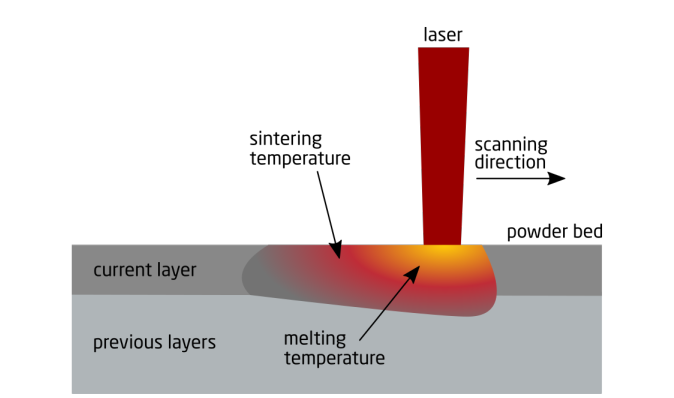
\includegraphics[width=0.9\textwidth]{Pictures/lpbf.png}
    \caption{The laser powder bed fusion process. A high power laser travels through a powder bed. Where the laser passes, the powder is melted, and as the laser moves on it solidifies again. This way 3D-components are manufactured additively, line-by-line. The figure is borrowed from Reference \cite[Fig. 2.4]{sebastian-phd} and reproduced with permission.}
    \label{fig:lpbf}
\end{figure}

The 3D-components are first created in CAD-software. This CAD-model is then passed on to a \textit{slicer} software together with a host of process parameters eg. the laser power and layer height. From the CAD-model and the process parameters the slicer calculates the appropriate instructions for the hardware. The hardware components are controlled by a microprocessor, called \textit{GLAMS}, which is fed with the commands by a \textit{g-code sender} software. The central hardware of the system are two mirrors mounted on galvanometers, in combination called a \textit{scanner}, and a lens. Galvanometers are electrical actuators that rotate an axis based on the current passing through their terminals. The scanner and the lens are used together to steer and focus the high power laser on the bed of metal powder, which then melts and hardens to create the layers of the print. For each layer of the print a new layer of feedstock is distributed on top of the previous layer. Figure \ref{fig:system-overview} shows an overview of the full system.

\begin{figure}
    \sffamily
    \centering
    \includesvg[width=\linewidth]{Pictures/system-overview.svg}
    \caption{An overview of the L-PBF system. The software components are marked in grey, the hardware components in purple. The "Etc." block represents small peripherals like cooling, camera, safety sensors etc. On the arrows, the text notes what file type or protocol is used to pass on information. Both "voltage" signals are variable 0-10V setpoint voltages.}
    \label{fig:system-overview}
\end{figure}

All research on this project was done with and for an existing L-PBF system, called Baxter, which is the result of the work in Reference \cite{sebastian-phd}, but broader applicability was kept in mind throughout the work.

\subsection{Software components}

The software components of the system have all been developed by the Open AM group. Here they are presented in a bit more detail:
\begin{itemize}
    \item \textbf{Slicer} The slicer reads a 3D-model in the form of an .stl file and takes process parameters as manual input. The model and parameters are then combined to calculate the layers of the print, or more specifically, the hatching and contour lines. These lines are then in turn converted to g-code commands which specify in full detail how the hardware components of the L-PBF need to move to obtain the desired end result. G-code is a programming language for computer-aided manufacturing. It is used to specify instructions for a controller that then activates the appropriate hardware to carry out these instructions. For this project the most relevant command is the instruction to move the mirrors to point the laser at a given set of coordinates. This command also includes a given speed at which to do the movement and a laser power (possibly off).
    \item \textbf{G-code sender} The only function of the g-code sender is to read the g-code and send it line-by-line to the printer at the pace it can process it.
    \item \textbf{GLAMS} GLAMS is the name for the micro controller that converts the g-code lines into control signals for the hardware. It is based on a Teensy microprocessor and has a wide range of I/O modules to control the laser, scanner etc. It works in real-time, reading and answering the g-code commands continuously, but it does have a small buffer.
\end{itemize}

\subsection{Hardware components}

Most of the hardware components are proprietary designs from industry suppliers. Their functions in the system are listed below, and the specific models of each of the main hardware components relevant to this project which are in use in Baxter at the time of writing are listed in Table \ref{tab:list-of-components}.

\begin{itemize}
    \item \textbf{Laser} The laser used in the system is a high power fibre laser. The beam has a wavelength of 1070 nm and the maximum power is 250 W
    \item \textbf{Beam expander} Before the laser reaches the scanner, it is passed through a beam expander. The laser source produces a very narrow beam with high energy density which would deteriorate the mirrors quickly. Therefore the beam expander is used to protect the mirrors. It widens the diameter of the beam, thus spreading the energy on a wider surface.
    \item \textbf{Scanner} The scanner, as described earlier, consists of two mirrors mounted on galvanometers. Positions of the mirrors are communicated to the scanner via the digital XY2-100 protocol, which is then converted to an analogue current signal which steers the galvanometers.
    \item \textbf{F-theta lens} After the (expanded) beam has passed through the scanner it is then focused again by a specific type of lens stack, namely an \textit{f-theta lens}. This lens brings the beam in focus at just the right height where the powder bed is. The optical properties are ensuring that even when the beam is pointed off-centre, meaning it travels a longer distance from the optics to the powder bed, the focal point is still at just the right height. Lastly the lens also works to ease the control of the system by directing the focus point in such a way that there in principle is a linear relation between the mirror angles and the position in the powder bed. More on this in Section \ref{sec:f-theta-model}.
    \item \textbf{Peripherals} The L-PBF system has a lot of peripheral components that fulfil important, but secondary functions. Those include a cooling system that prevents overheating of the scanner mirrors, a series of safety electronics that protect operators from being blinded or burned by the laser, a camera to look into the build chamber during the print and much more.
\end{itemize}

All the components are mounted in a chassis. The chassis includes a build chamber, where the manufacturing takes place. The chamber is sealed off during production, except for the ventilation cross-flow.

\begin{table}[h]
    \centering
    \begin{tabular}{l|l|c}
        Component & Model & Spec. sheet \\
        \hline
        Laser & SPI redPower R4.3 & \cite{laser-spec}\\
        Beam expander & Jenoptik Beam Expander 1x–8x Motorized & \cite{beam-expander-spec} \\
        Scanner & Scanlab intelliSCAN III 20 & \cite{scanner-spec} \\
        F-theta lens & JENar™ Silverline™ Lens 423-1030…1080-360 & \cite{f-theta-lens-spec}
    \end{tabular}
    \caption{List of primary components for Baxter, the L-PBF system in use for this project}
    \label{tab:list-of-components}
\end{table}
